\chapter{Neural Networks}
In this chapter, we discuss \href{https://en.wikipedia.org/wiki/Artificial_neural_network}{artificial neural networks}.
Many of the most visible breakthroughs in artificial intelligence have been achieved through the use of neural
networks: 
\begin{enumerate}
\item The current system used by Google to \href{https://translate.google.com}{automatically translate} web
      pages is called 
      ``\href{https://en.wikipedia.org/wiki/Google_Neural_Machine_Translation}{Google Neural Machine Translation}''
      and, as the name suggests, is based on neural networks. 
\item \href{https://www.deepl.com/translator}{DeepL} is another translator that is based on neural networks.      
\item \href{https://de.wikipedia.org/wiki/AlphaGo}{AlphaGo} uses neural networks together with tree search
      \cite{silver:2016}.  It has \href{https://en.wikipedia.org/wiki/AlphaGo_versus_Ke_Jie}{beaten} 
      beaten the world champion \href{https://en.wikipedia.org/wiki/Ke_Jie}{Ke Jie} in the game of
      \href{https://en.wikipedia.org/wiki/Go_(game)}{Go}. AlphaGo has been succeeded by
      \href{https://en.wikipedia.org/wiki/AlphaZero}{AlphaZero}, which is even stronger than AlphaGo.
\item \href{https://www.tensorflow.org/tutorials/image_recognition}{Image recognition} is best done via neural networks.
\item \href{https://en.wikipedia.org/wiki/Autonomous_car}{Autonomous driving} makes heavy use of neural networks.
\end{enumerate}
The list given above is far from being complete.  In this chapter, we will only discuss 
\href{https://en.wikipedia.org/wiki/Feedforward_neural_network}{feedforward neural networks}.  Although recently both 
\href{https://en.wikipedia.org/wiki/Convolutional_neural_network}{convolutional neural networks} and
\href{https://en.wikipedia.org/wiki/Recurrent_neural_network}{recurrent neural networks} have gotten a lot of
attention, these type of neural networks are more difficult to understand and are therefore beyond the scope of this
introduction.  The rest of this chapter is strongly influenced by the online book 
\\[0.2cm]
\hspace*{1.3cm}
\href{http://neuralnetworksanddeeplearning.com/index.html}{http://neuralnetworksanddeeplearning.com/index.html}
\\[0.2cm]
that has been written by Michael Nielsen \cite{nielsen:2015}.  This book is easy to read, carefully written, and
free to access.  I recommend this book to anybody who wants to dive deeper into the fascinating topic of neural
networks.  Furthermore, the online learning platform \href{https://www.coursera.org/}{Coursera} offers a
\blue{specialization} called \href{https://www.coursera.org/specializations/deep-learning}{Deep Learning} that
is exclusively devoted to neural networks.

We proceed to give an overview of the content of this chapter.
\begin{enumerate}
\item We start with the definition of \blue{feed forward} neural networks and discuss their \blue{topology}.
\item We introduce \blue{forward propagation}, which is the way a neural network computes its predictions.
\item Similarly to our treatment of logistic regression, we define a cost function that measure the quality of
      the predictions of a neural network on a training set.  In order to minimize this cost function using
      gradient descent, we have to compute the \blue{gradient} of the cost function with respect to the weights of the
      neural network.  The algorithm which is used to compute this gradient is called \blue{back propagation}.
\item In order to find the minimum of the cost function efficiently, we need an improved version of
      \blue{gradient descent}.  This improved version is known as \blue{stochastic gradient descent}.
\item After having covered the theory, we implement a simple neural network that is able to recognize
      handwritten digits.
\item Finally, we discuss \href{https://www.tensorflow.org}{TensorFlow}, which is an open source software
      library for machine learning in general and neural networks in particular.
\end{enumerate}

\section{Feedforward Neural Networks}
A neural network is built from \blue{neurons}.  Neural networks are inspired by biological 
\href{https://en.wikipedia.org/wiki/Neuron}{neurons}.  However, in order to understand artificial neural
networks it is not necessary to know how biological neurons work and it is definitely not necessary to
understand how networks of biological neurons, i.e.~brains, work\footnote{
  Actually, when it comes to brains, although there are many speculations, surprisingly little is known for a fact.  
}.  
Instead, we will use a mathematical abstraction of neurons that will serve as the foundation of the theory
developed in this chapter.  At the abstraction level that we are looking at neural networks, a single neuron
with $n$ inputs is specified by a pair $\langle \mathbf{w}, b\rangle$ where the vector $\mathbf{w} \in \mathbb{R}^m$ is called the \blue{weight vector} and 
the number $b \in \mathbb{R}$ is called the \blue{bias}.   
Conceptually, a neuron is a function that maps an input vector $\mathbf{x} \in \mathbb{R}^m$ into the set
$\mathbb{R}$ of the real numbers.  This function is defined as follows: 
\\[0.2cm]
\hspace*{1.3cm}
$\ds \mathbf{x} \mapsto a(\mathbf{x} \cdot \mathbf{w} + b)$.
\\[0.2cm]
Here, $a$ is called the \blue{activation function}.  In our applications, we will use the sigmoid
function as our activation function.  This function has been defined previously in Definition \ref{def:sigmoid}
on page \pageref{def:sigmoid} as follows:
\\[0.2cm]
\hspace*{1.3cm}
$\ds a(t) := S(t) = \frac{1}{1 + \exp(-t)}$.
\\[0.2cm]
Another useful activation function is the so called
\href{https://en.wikipedia.org/wiki/Rectifier_(neural_networks)}{ReLU function}, which is defined as 
\\[0.2cm]
\hspace*{1.3cm}
$a(t) = \max(0, x)$.
\\[0.2cm]
The abbreviation ReLU is short for \blue{rectified linear unit}.
The function modelling the neuron can be written more explicitly using index notation.  If
\\[0.2cm]
\hspace*{1.3cm}
$\mathbf{w} = \langle w_1, \cdots, w_m \rangle^\top$ 
\\[0.2cm]
is the weight vector and 
\\[0.2cm]
\hspace*{1.3cm}
$\mathbf{x} = \langle x_1, \cdots, x_m \rangle^\top$
\\[0.2cm]
is the input vector, then we have
\\[0.2cm]
\hspace*{1.3cm}
$\ds \mathbf{x} \mapsto S\left(\biggl(\sum\limits_{i=1}^m x_i \cdot w_i\biggr) + b\right)$.
\\[0.2cm]
If we compare this function to a similar function appearing in the last chapter, you will notice 
that a single neuron works just like a classifier in logistic regression.  The only difference is that the bias $b$
is now explicit in our notation.  In logistic regression, we had assumed that the first component $x_1$ of our
feature vector $\mathbf{x}$ was always equal to $1$.  This assumption enabled us to incorporate the bias $b$ into the
weight vector $\mathbf{w}$.

\begin{figure}[!h]
  \centering
   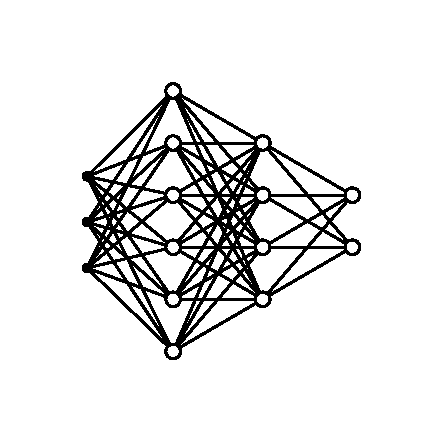
\epsfig{file=Figures/nn1.pdf,scale=1.5}
   \caption{A neural network with topology $[3, 6, 4, 2]$.}
  \label{fig:nn1.pdf}
\end{figure}

A \blue{feedforward neural network} is a layered network of neurons.  Formally, the \blue{topology} of a neural network is
given by a number $L \in \mathbb{N}$ and a list $[m(1), \cdots, m(L)]$ of $L$ natural numbers.  The number
$L$ is called the \blue{number of layers} and for $i \in \{2,\cdots,L\}$ the number $m(i)$ is the number of
neurons in the $l$-th layer.  The first layer is called the \blue{input layer}.  The input layer does not contain
neurons but instead just contains \blue{input nodes}.  The last layer (i.e.~the
layer with index $L$) is called the \blue{output layer} and the remaining layers are called 
\blue{hidden layers}.  If there is more than one hidden layer, the neural network is called a
\blue{deep neural network}.  Figure \ref{fig:nn1.pdf} on page \pageref{fig:nn1.pdf} shows
a small neural network with two hidden layers.  Including the input layer it has four layers and its topology
is given by the list $[3, 6, 4, 2]$.  A larger neural network with three hidden layers is shown in Figure
\ref{fig:nn2.pdf} on page \pageref{fig:nn2.pdf}.  I have written a small Jupyter notebook that can be used to
draw diagrams of this kind. This notebook is available at
\href{https://github.com/karlstroetmann/Artificial-Intelligence/blob/master/Python/NN-Architecture.ipynb}{NN-Architecture.ipynb}
in the \texttt{Python} subdirectory of my GitHub repository for this lecture. 


\begin{figure}[!h]
  \centering
   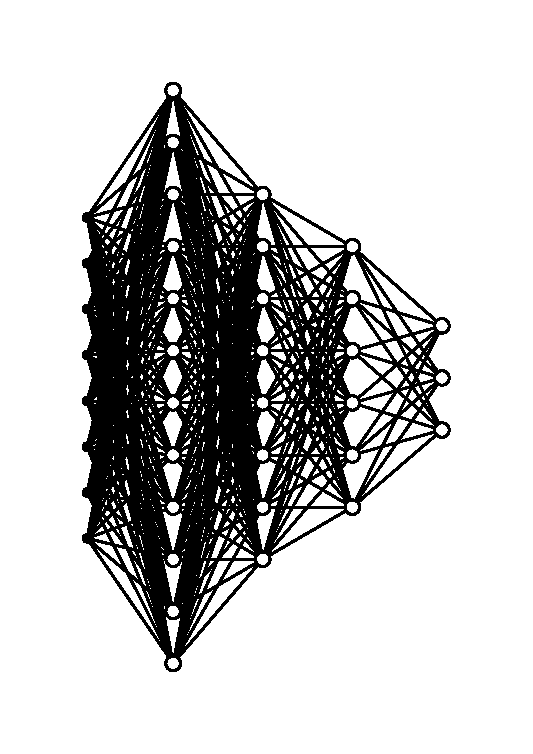
\epsfig{file=Figures/nn2.pdf,scale=1.5}
   \caption{A neural network with topology $[8, 12, 8, 6, 3]$.}
  \label{fig:nn2.pdf}
\end{figure}


If the topology of a neural network is  $[m(1), \cdots, m(L)]$, the \blue{input dimension} is defined as
$m(1)$.  Similarly, the \blue{output dimension} is defined as $m(L)$.
The feedforward neural networks discussed in this chapter are \blue{fully connected}:  Every node in the $l$-th
layer is connected to every node in the $(l+1)$-th layer via a \blue{weight}. 
The weight $w_{j,k}^{(l)}$ is the weight of the connection from the $k$-th neuron in layer $l-1$ to
the $j$-th neuron in layer $l$.  The weights in layer $l$ are combined into the \blue{weight matrix} $W^{(l)}$ of
the layer $l$: This matrix is defined as
\\[0.2cm]
\hspace*{1.3cm}
$\ds W^{(l)} := \bigl( w_{j,k}^{(l)} \bigr)$.
\\[0.2cm]
Note that $W^{(l)}$ is an $m(l) \times m(l-1)$ matrix, i.e.~we have
\\[0.2cm]
\hspace*{1.3cm}
$\ds W^{(l)} \in \mathbb{R}^{m(l) \times m(l-1)}$.
\\[0.2cm]
The $j$-th neuron in layer $l$ has the \blue{bias} $b_j^{(l)}$.  These biases of layer $l$ are combined into
the \blue{bias vector}
\\[0.2cm]
\hspace*{1.3cm}
$\mathbf{b}^{(l)} := \langle b_1^{(l)}, \cdots, b_{m(l)}^{(l)} \rangle^\top$.
\\[0.2cm]
The \blue{activation} of the $j$-th neuron
in layer $l$ is denoted as $a_j^{(l)}$ and is defined recursively as follows:
\begin{enumerate}
\item For the input layer we have
      \begin{equation}
        \label{eq:FF1}
       a^{(1)}_j(\mathbf{x}) := x_j.
       \tag{FF1}
      \end{equation}
      To put it differently, the input vector $\mathbf{x}$ is the activation of the input nodes.
\item For all other layers we have
      \begin{equation}
         \label{eq:FF2}
         a_j^{(l)}(\mathbf{x}) := 
             S\left(\Biggl(\sum\limits_{k=1}^{m(l-1)} w_{j,k}^{(l)}\cdot a_k^{(l-1)}(\mathbf{x})\Biggr) + b_{j}^{(l)}\right) 
        \quad \mbox{for all $l \in \{2, \cdots, L\}$}.
       \tag{FF2}
\end{equation}
\end{enumerate}
The \blue{activation vector} of layer $l$ is defined as
\\[0.2cm]
\hspace*{1.3cm}
$\mathbf{a}^{(l)}(\mathbf{x}) := \langle a_1^{(l)}(\mathbf{x}), \cdots, a_{m(l)}^{(l)}(\mathbf{x}) \rangle^\top$.
\\[0.2cm]
Using vector notation, the \blue{feed forward equations} (\ref{eq:FF1}) and (\ref{eq:FF2}) can be
rewritten as follows:
\begin{align}
  \label{eq:FF1v}
  \mathbf{a}^{(1)}(\mathbf{x}) & := \mathbf{x},
  \tag{FF1v} \\ 
  \label{eq:FF2v}
  \mathbf{a}^{(l)}(\mathbf{x}) & := 
  S\Bigl( W^{(l)} \cdot \mathbf{a}^{(l-1)}(\mathbf{x})\bigr) + \mathbf{b}^{(l)}\Bigr)
  \quad \mbox{for all $l \in \{2, \cdots, L\}$}.
  \tag{FF2v}
\end{align}

The output of our neural network for an input $\mathbf{x}$ is given by the neurons in the output
layer,  i.e.~the output vector 
$\mathbf{o}(\mathbf{x}) \in \mathbb{R}^{m(L)}$ is defined as 
\\[0.2cm]
\hspace*{1.3cm}
$\mathbf{o}(\mathbf{x}) := \langle a^{(L)}_1(\mathbf{x}), \cdots, a^{(L)}_{m(L)}(\mathbf{x}) \rangle^\top = \mathbf{a}^{(L)}(\mathbf{x})$.
\\[0.2cm]
Note that the equations (\ref{eq:FF1}) and (\ref{eq:FF2}) describe how information propagates
through the neural network: 
\begin{enumerate}
\item Initially, the input vector $\mathbf{x}$ is given and stored in the input layer of the neural network:
      \\[0.2cm]
      \hspace*{1.3cm}
      $\mathbf{a}^{(1)}(\mathbf{x}) := \mathbf{x}$.
\item The first layer of neurons, which is the second layer of nodes,  is activated and computes the activation
      vector $\mathbf{a}^{(2)}$ according to the formula
      \\[0.2cm]
      \hspace*{1.3cm}
      $\mathbf{a}^{(2)}(\mathbf{x}) := S\bigl(W^{(2)} \cdot \mathbf{a}^{(1)}(\mathbf{x}) + \mathbf{b}^{(2)}\bigr) = 
                                        S\bigl(W^{(2)} \cdot \mathbf{x} + \mathbf{b}^{(2)}\bigr)
      $.
\item The second layer of neurons, which is the third layer of nodes,  is activated and computes the activation
      vector $\mathbf{a}^{(3)}(\mathbf{x})$ according to the formula
      \\[0.2cm]
      \hspace*{1.3cm}
      $\mathbf{a}^{(3)}(\mathbf{x}) := S\bigl(W^{(3)} \cdot \mathbf{a}^{(2)}(\mathbf{x}) + \mathbf{b}^{(3)}\bigr)
                          = S\Bigl(W^{(3)} \cdot S\bigl(W^{(2)} \cdot \mathbf{x} + \mathbf{b}^{(2)}\bigr) + \mathbf{b}^{(3)}\Bigr)
        $
\item This proceeds until the output layer is reached and the output
      \\[0.2cm]
      \hspace*{1.3cm}
      $\mathbf{o}(\mathbf{x}) := \mathbf{a}^{(L)}(\mathbf{x})$
      \\[0.2cm]
      has been computed.  As long as we use the sigmoid function as our activation function, every neuron of
      the neural network performs logistic regression. 
\end{enumerate}
Next, we assume that we have $n$ \blue{training examples} 
\\[0.2cm]
\hspace*{1.3cm}
$\langle \mathbf{x}^{(i)}, \mathbf{y}^{(i)} \rangle$ \quad for $i=1,\cdots,n$ 
\\[0.2cm]
such that 
\\[0.2cm]
\hspace*{1.3cm}
$\mathbf{x}^{(i)} \in \mathbb{R}^{m(1)}$ and $\mathbf{y}^{(i)} \in \mathbb{R}^{m(L)}$.
\\[0.2cm]
Our goal is to choose the weight matrices $W^{(l)}$ and the bias vectors $\mathbf{b}^{(l)}$ in a way such that
\\[0.2cm]
\hspace*{1.3cm}
$\mathbf{o}\bigl(\mathbf{x}^{(i)}\bigr) = \mathbf{y}^{(i)}$ \quad for all $i \in \{1,\cdots,n\}$.
\\[0.2cm]
Unfortunately, in general we will not be able to achieve equality for all  $i \in \{1,\cdots,n\}$.
Therefore, our goal is to minimize the \blue{error} instead.  To be more precise, the 
\blue{quadratic error cost function} is defined as 
\\[0.2cm]
\hspace*{1.3cm}
$\ds C\Bigr(W^{(2)}, \cdots, W^{(L)}, \mathbf{b}^{(2)}, \cdots, \mathbf{b}^{(L)};
     \mathbf{x}^{(1)}, \mathbf{y}^{(1)}, \cdots, \mathbf{x}^{(n)},\mathbf{y}^{(n)} \Bigr) := 
 \frac{1}{2 \cdot n} \cdot \sum\limits_{i=1}^n \Bigl(\mathbf{o}\bigl(\mathbf{x}^{(i)}\bigr) - \mathbf{y}^{(i)}\Bigr)^2
$.
\\[0.2cm]
Note that this cost function is additive in the training examples $\langle \mathbf{x}^{(i)}, \mathbf{y}^{(i)} \rangle$.
In order to simplify the notation we define
\\[0.2cm]
\hspace*{1.3cm}
$\ds C_{\mathbf{x}, \mathbf{y}}\Bigr(W^{(2)}, \cdots, W^{(L)}, \mathbf{b}^{(2)}, \cdots, \mathbf{b}^{(L)}\Bigr) := 
 \frac{1}{2} \cdot \Bigl(\mathbf{a}^{(L)}\bigl(\mathbf{x}\bigr) - \mathbf{y}\Bigr)^2
$,
\\[0.2cm]
i.e.~$C_{\mathbf{x},\mathbf{y}}$ is the part of the cost function that is associated with a single training example $\pair(\mathbf{x},\mathbf{y})$.
Then, we have
\\[0.2cm]
$\ds C\Bigr(W^{(2)}, \cdots, W^{(L)}, \mathbf{b}^{(2)}, \cdots, \mathbf{b}^{(L)};
     \mathbf{x}^{(1)}, \mathbf{y}^{(1)}, \cdots, \mathbf{x}^{(n)},\mathbf{y}^{(n)} \Bigr) := 
 \frac{1}{n} \cdot \sum\limits_{i=1}^n C_{\mathbf{x^{(i)}}, \mathbf{y}^{(i)}}\Bigr(W^{(2)}, \cdots W^{(L)}, \mathbf{b}^{(2)}, \cdots, \mathbf{b}^{(L)}\Bigr) 
$.
\\[0.2cm]
As the notation
\\[0.2cm]
\hspace*{1.3cm}
$C_{\mathbf{x}, \mathbf{y}}\Bigr(W^{(2)}, \cdots, W^{(L)}, \mathbf{b}^{(2)}, \cdots, \mathbf{b}^{(L)}\Bigr)$
\\[0.2cm]
is far too heavy, we will abbreviate this term as $C_{\mathbf{x}, \mathbf{y}}$ in the following
discussion of the backpropagation algorithm.  Similarly, we abbreviate the quadratic error cost function as $C$.
Our goal is to choose the weight matrices $W^{(l)}$ and the bias vectors $\mathbf{b}^{(l)}$ such that the
quadratic error cost function $C$ is minimized.  We will use a variation of gradient descent to
find this minimum\footnote{
  In logistic regression we have tried to \emph{maximize} the log-likelihood.  Here, instead
  we \emph{minimize} the quadratic error cost function.  Hence, instead of gradient \emph{ascent} we use
  gradient \emph{descent}.  
}.
Unfortunately, the cost function $C$ when regarded as a function of the weights and biases has many local 
minima.  Hence, in practical applications all we can hope for is to find a local minimum that is good enough
for the goal that we want to achieve.


\section{Backpropagation}
There are three reasons for the recent success of neural networks.
\begin{enumerate}
\item The computing power that is available today has vastly increased in the last 20 years.
      For example, today the \href{https://en.wikipedia.org/wiki/AMD_RX_Vega_series}{AMD Radeon Vega \texttt{VII}}
      graphic card offers about 13.8 teraflops in single precision performance.  It consumes about 300 watt.
      Contrast this with \href{https://en.wikipedia.org/wiki/ASCI_White}{ASCI White}, which was the most powerful supercomputer in 2000:
      According to the article ``\href{https://en.wikipedia.org/wiki/History_of_supercomputing}{History of Supercomputing}'', 
      it  offered a performance of 7.2 teraflops.  It needed 6 megawatt to operate.  The cost to build ASCI White was about $110,000,000\,\symbol{36}$.
      To compare, the AMD RX Vega \texttt{VII} costs $699\,\symbol{36}$.

      The Nvidia \href{https://www.nvidia.com/en-us/titan/titan-v/}{Titan V} comes at $2,999\,\symbol{36}$ and
      offers a stunning 110 teraflops for \href{https://en.wikipedia.org/wiki/Deep_learning}{deep learning} via
      the \href{https://en.wikipedia.org/wiki/CUDA}{\textsc{Cuda}} \textsc{Api}.
\item The breakthrough in the theory of neural networks was the rediscovering of the
      \href{https://en.wikipedia.org/wiki/Backpropagation}{backpropagation algorithm} by
      David Rumelhart, Geoffrey Hinton, and Ronald Williams \cite{rumelhart:1986} in 1986.  
      The backpropagation algorithm had first been discovered by Arthur E.~Bryson, Jr.~and Yu-Chi Ho
      \cite{bryson:1969}.  In recent years, there have been a number of other theoretical advances that have
      helped in speeding up the learning algorithms for neural networks.
\item Lastly, as neural networks have large sets of parameters, they need large sets of training examples.  The
      recent digitization of our society has made these large data sets available.
\end{enumerate}
Essentially, the \blue{backpropagation} algorithm is an efficient way to compute the partial derivatives of the
cost function $C$ with respect to the weights $w_{j,k}^{(l)}$ and the biases $b_j^{(l)}$.  Before we can
proceed to compute these partial derivatives, we need to define some auxiliary variables. 

\subsection{Definition of some Auxiliary Variables}
We start by defining the auxiliary variables $z_j^{(l)}$.
 The expressions $z_j^{(l)}$  are defined as the inputs of the activation function $S$ of the $j$-th neuron in
 layer $l$:
\\[0.2cm]
\hspace*{1.3cm}
$\ds z_j^{(l)} := \left(\sum\limits_{k=1}^{m(l-1)}  w_{j,k}^{(l)} \cdot a_k^{(l-1)}\right) + b_j^{(l)}$
\quad for all  $j \in \{1, \cdots, m(l)\}$ and $l \in \{2,\cdots,L\}$.
\\[0.2cm]
Of course, the term  $a_k^{(l-1)}$ really is a function of the input vector $\mathbf{x}$.  However, it is better to suppress
this dependence in the notation since otherwise the formul\ae\ get too cluttered.
Essentially, $z_j^{(l)}$ is the input to the sigmoid function when the activation $a_j^{(l)}$ is computed,
i.e.~we have
\\[0.2cm]
\hspace*{1.3cm}
$a_j^{(l)} = S\Bigl(z_j^{(l)}\Bigr)$.
\\[0.2cm]
Later, we will see that the partial derivatives of the cost function $C_{\mathbf{x}, \mathbf{y}}$ with respect to both the weights
$w_{j,k}^{(l)}$ and the biases $b_j^{(l)}$ can be computed easily if we first compute the partial derivatives
of $C_{\mathbf{x}, \mathbf{y}}$ with respect to $z_j^{(l)}$.  Therefore we define
\\[0.2cm]
\hspace*{1.3cm}
$\ds\varepsilon_j^{(l)} := \frac{\partial C_{\mathbf{x}, \mathbf{y}}}{\partial z_j^{(l)}}$ \quad for all $j \in \{1, \cdots, m(l)\}$ and $l \in \{2,\cdots, L\}$,
\\[0.2cm]
that is we regard $C_{\mathbf{x}, \mathbf{y}}$ as a function of the $z_j^{(l)}$ and take the partial
derivatives according to these variables.  
Note that $\varepsilon_j^{(l)}$ does depend on both $\mathbf{x}$ and $\mathbf{y}$.  
We call  $\varepsilon_j^{(l)}$ the \blue{error in the $j$-th neuron in the $l$-th layer}. 
Since the notation would
get too cumbersome if we would write this as $\varepsilon(\mathbf{x}, \mathbf{y})_j^{(l)}$, we regard the training
example $\langle\mathbf{x}, \mathbf{y}\rangle$ as fixed for now.  Next, the quantities $\varepsilon_j^{(l)}$ are combined into a vector:
\\[0.2cm]
\hspace*{1.3cm}
$\boldsymbol{\varepsilon}^{(l)} := \left(
  \begin{array}[c]{c}
    \varepsilon_1^{(l)}      \\
    \vdots             \\
    \varepsilon_{m(l)}^{(l)}  
  \end{array}
  \right)
$.
\\[0.2cm]
The vector $\boldsymbol{\varepsilon}^{(l)}$ is called the \blue{error in layer $l$}.

\subsection{The Hadamard Product}
Later, we will have need of the \href{https://en.wikipedia.org/wiki/Hadamard_product_(matrices)}{Hadamard product} 
of two vectors.  Assume that $\mathbf{x}, \mathbf{y} \in \mathbb{R}^n$.  The \blue{Hadamard product} of
$\mathbf{x}$ and $\mathbf{y}$ is a \blue{vector} that is defined by multiplying the vectors $\mathbf{x}$ and $\mathbf{y}$ elementwise:
\\[0.2cm]
\hspace*{1.3cm}
$\left(
  \begin{array}[c]{c}
    x_1 \\
    x_2 \\
    \vdots \\
    x_n
  \end{array}
\right) \odot
\left(
  \begin{array}[c]{c}
    y_1 \\
    y_2 \\
    \vdots \\
    y_n
  \end{array}
\right) := 
\left(
  \begin{array}[c]{c}
    x_1 \cdot y_1 \\
    x_2 \cdot y_2 \\
    \vdots \\
    x_n \cdot y_n
  \end{array}
\right)
$,
\\[0.2cm]
i.e.~the $i$-th component of the Hadamard product $\mathbf{x} \odot \mathbf{y}$ is the product of the $i$-th
component of $\mathbf{x}$ with the $i$-th component of $\mathbf{y}$.  Do not confuse the Hadamard product with
the \href{https://en.wikipedia.org/wiki/Dot_product}{dot product}!  Although both multiply the vectors
componentwise, the Hadamard product returns a vector, while the dot product returns a number.  Later, we will
use the \href{http://www.numpy.org}{NumPy} package to represent vectors.  In NumPy, the Hadamard product of two
vectors $\mathtt{x}$ and $\mathtt{y}$ is computed by the expression $\mathtt{x} * \mathtt{y}$.

\subsection{Backpropagation: The Equations}
Now we are ready to state the \blue{backpropagation equations}.  The first of these four equations reads as follows:
\begin{equation}
  \label{eq:BP1}
  \varepsilon^{(L)}_j = (a_j^{(L)} - y_j) \cdot S'\bigl(z_j^{(L)}\bigr)
 \quad \mbox{for all $j \in \{1, \cdots, m(L)\}$,}
  \tag{BP1}
\end{equation}
where $S'(x)$ denotes the derivative of the sigmoid function.  We have shown in Chapter
\ref{chapter:classification} that this derivative satisfies the equation
\\[0.2cm]
\hspace*{1.3cm}
$S'(t) = \bigl(1 - S(t)\bigr) \cdot S(t)$.
\\[0.2cm]
The equation (\ref{eq:BP1}) can also be written in vectorized form using the Hadamard product:
\begin{equation}
  \label{eq:BP1s}
\boldsymbol{\varepsilon}^{(L)} = (\mathbf{a}^{(L)} - \mathbf{y}) \odot S'\bigl(\mathbf{z}^{(L)}\bigr)  
\tag{BP1v}
\end{equation}
Here, we have \blue{vectorized} the application of the function $S'$ to the vector $\mathbf{z}^{(L)}$, i.e.~the
expression $S'\bigl(\mathbf{z}^{(L)}\bigr)$ is defined as follows:
\\[0.2cm]
\hspace*{1.3cm}
$ S'\left(
  \begin{array}[c]{c}
   z_1^{(L)}      \\
   \vdots       \\
   z_{m(L)}^{(L)} 
  \end{array}
  \right) := \left(
  \begin{array}[c]{c}
   S'\bigl(z_1^{(L)}\bigr)      \\
   \vdots       \\
   S'\bigl(z_{m(L)}^{(L)}\bigr)
  \end{array}
  \right)
$.
\\[0.2cm]
The next equation computes $\varepsilon_j^{(l)}$ for $l < L$.  
\begin{equation}
  \label{eq:BP2}
  \varepsilon^{(l)}_j = \sum\limits_{i=1}^{m(l+1)} w_{i,j}^{(l+1)} \cdot \varepsilon^{(l+1)}_i \cdot
  S'\bigl(z^{(l)}_j\bigr) \quad \mbox{for all $j \in \{1, \cdots, m(l)\}$ and $l \in \{2, \cdots, L-1\}$}.
  \tag{BP2}
\end{equation}
This equation is more succinct in vectorized notation:
\begin{equation}
  \label{eq:BP2v}
  \boldsymbol{\varepsilon}^{(l)} = \Bigl(\bigl(W^{(l+1)}\bigr)^\top \cdot \boldsymbol{\varepsilon}^{(l+1)}\Bigr) \odot
  S'\bigl(\mathbf{z}^{(l)}\bigr) \quad \mbox{for all $l \in \{2, \cdots, L-1\}$}.
  \tag{BP2v}
\end{equation}
Note that this equation computes the error in layer $l$ for $l < L$ in terms
of the error in layer $l+1$:  The error 
$\boldsymbol{\varepsilon}^{(l+1)}$ at layer $l+1$ is \blue{propagated backwards} through the neural network to produce the
error $\boldsymbol{\varepsilon}^{(l)}$ at layer $l$.  This is the reason for calling the associated algorithm \blue{backpropagation}.

Next, we have to compute the partial derivative of $C_{\mathbf{x}, \mathbf{y}}$ with respect to the bias of the
$j$-th neuron in layer $l$, which is denoted as $b_j^{(l)}$.  We have
\begin{equation}
  \label{eq:BP3}
  \frac{\partial C_{\mathbf{x}, \mathbf{y}}}{\partial b_j^{(l)}} = \varepsilon_j^{(l)}
  \quad \mbox{for all $j \in \{1,\cdots,m(l)\}$ and $l \in \{2, \cdots,L\}$.}
  \tag{BP3}
\end{equation}
This equation shows the reason for defining the error terms $\varepsilon_j^{(l)}$.
In vectorized notation, this equation takes the following form:
\begin{equation}
  \label{eq:BP3v}
  \nabla_{\mathbf{b}^{(l)}} C_{\mathbf{x}, \mathbf{y}} = \boldsymbol{\varepsilon}^{(l)}
  \quad \mbox{for all $l \in \{2, \cdots,L\}$.}
  \tag{BP3v}
\end{equation}
Here, $\nabla_{\mathbf{b}^{(l)}} C_{\mathbf{x}, \mathbf{y}}$ denotes the gradient of $C_{\mathbf{x},
  \mathbf{y}}$ with respect to the bias vector $\mathbf{b}^{(l)}$.
Finally, we can compute the  partial derivative of $C_{\mathbf{x}, \mathbf{y}}$ with respect to the weights $w_{j,k}^{(l)}$:
\begin{equation}
  \label{eq:BP4}
  \frac{\partial C_{\mathbf{x}, \mathbf{y}}}{\partial w_{j,k}^{(l)}} = \varepsilon_j^{(l)} \cdot a_k^{(l-1)} 
  \quad \mbox{for all $j \in \{1,\cdots,m(l)\}$, $ k \in \{1,\cdots,m(l-1)\}$, and $l \in \{2, \cdots,L\}$.}
  \tag{BP4}
\end{equation}
In vectorized notation, this equation can be written as:
\begin{equation}
  \label{eq:BP4v}
  \nabla_{W^{(l)}} C_{\mathbf{x}, \mathbf{y}} = \boldsymbol{\varepsilon}^{(l)} \cdot \bigl(\mathbf{a}^{(l-1)}\bigr)^\top
  \quad \mbox{for all $l \in \{2, \cdots,L\}$.}
  \tag{BP4v}
\end{equation}
Here, the expression $\boldsymbol{\varepsilon}^{(l)} \cdot \bigl(\mathbf{a}^{(l-1)}\bigr)^\top$ denotes the matrix
product of the column vector $\boldsymbol{\varepsilon}^{(l)}$ that is regarded as an $m(l) \times 1$ matrix and the
row vector $\bigl(\mathbf{a}^{(l-1)}\bigr)^\top$ that is regarded as an $1 \times m(l-1)$ matrix.

As the backpropagation equations are at the very core of the theory of neural networks, we highlight the
vectorized form of these equations:
\\[0.2cm]
\hspace*{0.3cm}
\colorbox{red}{\framebox{\colorbox{orange}{
\begin{minipage}[h]{0.92\linewidth}
$
\begin{array}[h]{llr}
  \ds \boldsymbol{\varepsilon}^{(L)} = (\mathbf{a}^{(L)} - \mathbf{y}) \odot S'\bigl(\mathbf{z}^{(L)}\bigr)
     & & \mbox{\hspace*{4cm}(BP1v)}  \\[0.2cm]
  \ds \boldsymbol{\varepsilon}^{(l)} = \Bigl(\bigl(W^{(l+1)}\bigr)^\top \cdot \boldsymbol{\varepsilon}^{(l+1)}\Bigr) \odot
  S'\bigl(\mathbf{z}^{(l)}\bigr) & \mbox{for all $l \in \{2, \cdots, L-1\}$} &
  \mbox{(BP2v)}  \\[0.3cm]
  \ds \nabla_{\mathbf{b}^{(l)}} C_{\mathbf{x}, \mathbf{y}} = \boldsymbol{\varepsilon}^{(l)}
  & \mbox{for all $l \in \{2, \cdots,L\}$}
  & \mbox{(BP3v)}
  \\[0.2cm]
  \ds \nabla_{W^{(l)}} C_{\mathbf{x}, \mathbf{y}} = \boldsymbol{\varepsilon}^{(l)} \cdot \bigl(\mathbf{a}^{(l-1)}\bigr)^\top
  & \mbox{for all $l \in \{2, \cdots,L\}$}
  & \mbox{(BP4v)}
\end{array}
$
\end{minipage}
}}}
\\[0.2cm]
The equations (\ref{eq:BP3}) and (\ref{eq:BP4}) show why it was useful to introduce the
vectors $\boldsymbol{\varepsilon}^{(l)}$: These vectors enable us to compute the partial derivatives of the cost function
with respect to both the biases and the weights.  The equations (\ref{eq:BP1}) and (\ref{eq:BP2})
show how the vectors $\boldsymbol{\varepsilon}^{(l)}$ can be computed.  An implementation of backpropagation should use the vectorized
versions of these equations since this is more efficient for two reasons:
\begin{enumerate}
\item Interpreted languages like \textsl{Python} take much more time to
      execute a loop than to execute a simple matrix-vector multiplication.  The reason is that in a loop, in
      addition to executing the statement a given number of times, the statement has to be interpreted 
      every time it is executed.
\item Languages that are optimized for machine learning often take care to delegate the execution of matrix
      operations to highly optimized functions that have been written in more efficient low level languages like
      \texttt{C} or assembler.  Often, these functions are able to utilize all cores of the processor
      simultaneously.  Furthermore, sometimes these functions can even use the graphical coprocessor
      which, because of parallelization, can do a matrix multiplication much faster than the floating point unit of
      a conventional processor.
\end{enumerate}

\subsection{A Proof of the Backpropagation Equations}
Since we are living in a time of fake news and alternative facts where
\href{https://www.theguardian.com/us-news/2018/aug/19/truth-isnt-truth-rudy-giuliani-trump-alternative-facts-orwellian}{truth isn't truth} 
and not even a president can be trusted,  you should not lightly believe the validity of the backpropagation equations.  Instead, 
we have to \textbf{prove} the backpropagation equations.  Although the proof is a bit tedious, it should be
accessible: We only need the \href{https://en.wikipedia.org/wiki/Chain_rule}{chain rule} from calculus and the 
\href{https://en.wikipedia.org/wiki/Chain_rule}{chain rule} from \href{https://en.wikipedia.org/wiki/Multivariable_calculus}{multivariate calculus}.

Lets us start with the proof of equations \ref{eq:BP1}.
Remember that we have defined the numbers $\varepsilon_j^{(l)}$ as
\\[0.2cm]
\hspace*{1.3cm}
$\ds\varepsilon_j^{(l)} = \frac{\partial C_{\mathbf{x}, \mathbf{y}}}{\partial z_j^{(l)}}$,
\\[0.2cm]
while the numbers $z_j^{(l)}$ have been defined as
\\[0.2cm]
\hspace*{1.3cm}
$\ds z_j^{(l)} := \left(\sum\limits_{k=1}^{m(l-1)}  w_{j,k}^{(l)} \cdot a_k^{(l-1)}(\mathbf{x})\right) + b_j^{(l)}$.
\\[0.2cm]
Since the quadratic error cost function $C_{\mathbf{x}, \mathbf{y}}$ for the training example $\pair(\mathbf{x}, \mathbf{y})$ has been defined 
in terms of the activation $\mathbf{a}^{(L)}(\mathbf{x})$ as 
\\[0.2cm]
\hspace*{1.3cm}
$\ds C_{\mathbf{x}, \mathbf{y}} = \frac{1}{2} \cdot \bigl(\mathbf{a}^{(L)}(\mathbf{x}) - \mathbf{y}\bigr)^2$
\\[0.2cm]
and we have $\mathbf{a}^{(L)}(\mathbf{x}) = S\bigl(\mathbf{z}^{(L)}\bigr)$, the chain rule of calculus tells us that $\varepsilon_j^{(L)}$ 
can be computed as follows:
\\[0.2cm]
\hspace*{1.3cm}
$
\begin{array}{lcll}
\varepsilon_j^{(L)} 
& = & \ds \frac{\partial C_{\mathbf{x}, \mathbf{y}}}{\partial z_j^{(L)}} \\[0.5cm]
& = & \ds \frac{\partial \quad}{\partial z_j^{(L)}}  \frac{1}{2} \cdot \bigl(\mathbf{a}^{(L)}(\mathbf{x}) - \mathbf{y}\bigr)^2
      \\[0.5cm]
& = & \ds \frac{1}{2} \cdot \frac{\partial \quad}{\partial z_j^{(L)}} 
      \sum\limits_{i=1}^{m(L)} \Bigl(a_i^{(L)}(\mathbf{x}) - y_i\Bigr)^2
      \\[0.5cm]
& = & \ds \frac{1}{2} \cdot \frac{\partial \quad}{\partial z_j^{(L)}} 
      \sum\limits_{i=1}^{m(L)} \Bigl(S\bigl(z_i^{(L)}\bigr) - y_i\Bigr)^2
      \\[0.5cm]
& = & \ds \frac{1}{2} \cdot
      \sum\limits_{i=1}^{m(L)} 2 \cdot \Bigl(S\bigl(z_i^{(L)}\bigr) - y_i\Bigr) \cdot 
      \frac{\partial \quad}{\partial z_j^{(L)}}S\bigl(z_i^{(L)}\bigr)
      \\[0.5cm]
& = & \ds \sum\limits_{i=1}^{m(L)} \Bigl(S\bigl(z_i^{(L)}\bigr) - y_i\Bigr) \cdot 
      S'\bigl(z_i^{(L)}\bigr) \cdot \frac{\partial z_i^{(L)}}{\partial z_j^{(L)}}

      \\[0.5cm]
& = & \ds \sum\limits_{i=1}^{m(L)} \Bigl(S\bigl(z_i^{(L)}\bigr) - y_i\Bigr) \cdot 
      S'\bigl(z_i^{(L)}\bigr) \cdot \delta_{i,j}
      & \mbox{$\delta_{i,j}$ denotes the \href{https://en.wikipedia.org/wiki/Kronecker\_delta}{Kronecker delta}}
      \\[0.5cm]
& = & \ds \Bigl(S\bigl(z_j^{(L)}\bigr) - y_j\Bigr) \cdot S'\bigl(z_j^{(L)}\bigr) 
      \\[0.5cm]
& = & \ds \Bigl(a_j^{(L)} - y_j\Bigr) \cdot S'\bigl(z_j^{(L)}\bigr) 
\end{array}
$
\\[0.2cm]
Thus we have proven equation \ref{eq:BP1}.  

We proceed to prove equation \ref{eq:BP2}.  To this end we compute $\varepsilon_j^{(l)}$ for $l < L$.  
This time, we need the chain rule of multivariate calculus.  As a reminder, the chain rule in multivariate calculus
works as follows: Assume that the functions
\\[0.2cm]
\hspace*{1.3cm}
$f: \mathbb{R}^k \rightarrow \mathbb{R}$ \quad and \quad
$g: \mathbb{R}^n \rightarrow \mathbb{R}^k$. 
\\[0.2cm]
are differentiable\footnote{
  If this text had been written in German, I would have said that $f$ and $g$ are ``\blue{total differenzierbar}''.
}.  
If the function $h: \mathbb{R}^n \rightarrow \mathbb{R}$ is defined as
\\[0.2cm]
\hspace*{1.3cm}
$h(\mathbf{x}) := f\bigl(g(\mathbf{x})\bigr)$ \quad for all $\mathbf{x} \in \mathbb{R}^n$,
\\[0.2cm]
then the partial derivative of $h$ with respect to $x_j$ satisfies
\\[0.2cm]
\hspace*{1.3cm}
$\ds \frac{\partial h}{\partial x_j} = 
 \sum\limits_{i=1}^k \frac{\partial f}{\partial y_i} \cdot \frac{\partial g_i}{\partial x_j}
$.
\\[0.2cm]



We have
\\[0.2cm]
\hspace*{1.3cm}
$
\begin{array}{lcll}
\varepsilon_j^{(l)} 
& = & \ds \frac{\partial C_{\mathbf{x}, \mathbf{y}}}{\partial z_j^{(l)}} \\[0.5cm]
& = & \ds \sum\limits_{i=1}^{m(l+1)} 
      \frac{\partial C_{\mathbf{x}, \mathbf{y}}}{\partial z_i^{(l+1)}} \cdot \frac{\partial z_i^{(l+1)}}{\partial z_j^{(l)}}
    & \mbox{using the chain rule of multivariate calculus}
      \\[0.5cm]
& = & \ds \sum\limits_{i=1}^{m(l+1)} 
      \varepsilon_i^{(l+1)} \cdot \frac{\partial z_i^{(l+1)}}{\partial z_j^{(l)}}
      & \mbox{using the definition of $\varepsilon_i^{(l+1)}$}     
\end{array}
$
\\[0.2cm]
In order to proceed, we have to remember the definition of $z_i^{(l+1)}$.  We have
\\[0.2cm]
\hspace*{1.3cm}
$\ds z_i^{(l+1)} = \left(\sum\limits_{k=1}^{m(l)} w_{i,k}^{(l+1)} \cdot S\bigl(z_k^{(l)}\bigr)\right) + b_i^{(l+1)}$
\\[0.2cm]
Therefore, the partial derivatives $\ds\frac{\partial z_i^{(l+1)}}{\partial z_j^{(l)}}$ 
can be computed as follows:
\\[0.2cm]
\hspace*{1.3cm}
$
\begin{array}{lcl}
      \ds \frac{\partial z_i^{(l+1)}}{\partial z_j^{(l)}} 
& = & \ds \sum\limits_{k=1}^{m(l)} 
      w_{i,k}^{(l+1)} \cdot S'\bigl(z_k^{(l)}\bigr) \cdot \frac{\partial z_k^{(l)}}{\partial z_j^{(l)}} 
      \\[0.5cm]
& = & \ds \sum\limits_{k=1}^{m(l)} 
      w_{i,k}^{(l+1)} \cdot S'\bigl(z_k^{(l)}\bigr) \cdot \delta_{k,j}
      \\[0.5cm]
& = & \ds w_{i,j}^{(l+1)} \cdot S'\bigl(z_j^{(l)}\bigr) 
\end{array}
$
\\[0.2cm]
If we substitute this expression back into the result we got for $\varepsilon_j^{(l)}$ we have shown the following:
\\[0.2cm]
\hspace*{1.3cm}
$
\begin{array}{lcll}
\varepsilon_j^{(l)} 
& = & \ds \sum\limits_{i=1}^{m(l+1)} 
      \varepsilon_i^{(l+1)} \cdot \frac{\partial z_i^{(l+1)}}{\partial z_j^{(l)}}
      \\[0.5cm]
& = & \ds \sum\limits_{i=1}^{m(l+1)} 
      \varepsilon_i^{(l+1)} \cdot w_{i,j}^{(l+1)} \cdot S'\bigl(z_j^{(l)}\bigr) 
      \\[0.5cm]
& = & \ds \sum\limits_{i=1}^{m(l+1)} 
      w_{i,j}^{(l+1)} \cdot \varepsilon_i^{(l+1)} \cdot S'\bigl(z_j^{(l)}\bigr) 
\end{array}
$
\\[0.2cm]
Therefore, we have now proven equation (\ref{eq:BP2}).  

We proceed to prove equation (\ref{eq:BP4}).  
According to the chain rule we have
\\[0.2cm]
\hspace*{1.3cm}
$ \ds\frac{\partial C_{\mathbf{x}, \mathbf{y}}}{\partial w_{j,k}^{(l)}}  =  
  \frac{\partial C_{\mathbf{x}, \mathbf{y}}}{\partial z_j^{(l)}} \cdot \frac{\partial z_j^{(l)}}{\partial w_{j,k}^{(l)}} 
$ 
\\[0.2cm]
Now by definition of $\varepsilon_j^{(l)}$, the first factor on the right hand side of this equation is equal to $\varepsilon_j^{(l)}$: 
\\[0.2cm]
\hspace*{1.3cm}
$\ds \varepsilon_j^{(l)} = \frac{\partial C_{\mathbf{x}, \mathbf{y}}}{\partial z_j^{(l)}}$.
\\[0.0cm]
In order to proceed, we need to evaluate the partial derivative
$\ds\frac{\partial z_j^{(L)}}{\partial w_{j,k}^{(l)}}$.  The term $z_j^{(l)}$ has been defined as follows:
\\[0.2cm]
\hspace*{1.3cm}
$\ds z_j^{(l)} = \left(\sum\limits_{k=1}^{m(l)} w_{j,k}^{(l)} \cdot S\bigl(z_k^{(l-1)}\bigr)\right) + b_j^{(l)}$.
\\[0.2cm]
Hence we have
\\[0.2cm]
\hspace*{1.3cm}
$\ds\frac{\partial z_j^{(l)}}{\partial w_{j,k}^{(l)}} = S\bigl(z_k^{(l-1)}\bigr) = a_k^{(l-1)}$. 
\\[0.2cm]
Combining these equations we arrive at
\\[0.2cm]
\hspace*{1.3cm}
$ \ds\frac{\partial C_{\mathbf{x}, \mathbf{y}}}{\partial w_{j,k}^{(l)}}  =  
  a_k^{(l-1)} \cdot \varepsilon_j^{(l)} 
$. 
\\[0.2cm]
Therefore, equation (\ref{eq:BP4}) has been verified.

\exercise
Prove equation (\ref{eq:BP3}).
\eoxs

\section{Stochastic Gradient Descent}
The equations describing backpropagation describe the gradient of the cost function for a single training
example $\pair(\mathbf{x}, \mathbf{y})$.  However, when we train a neural network, we need to take all training
examples into account.  If we have $n$ training examples
\\[0.2cm]
\hspace*{1.3cm}
$\langle\mathbf{x}^{(1)}, \mathbf{y}^{(1)})\rangle$,
$\langle\mathbf{x}^{(2)}, \mathbf{y}^{(2)})\rangle$,
$\cdots$,
$\langle\mathbf{x}^{(n)}, \mathbf{y}^{(n)})\rangle$,
\\[0.2cm]
then the quadratic error cost function has been previously defined as the sum
\\[0.2cm]
\hspace*{1.3cm}
$\ds C\Bigr(W^{(2)}, \cdots, W^{(L)}, \mathbf{b}^{(2)}, \cdots, \mathbf{b}^{(L)};
     \mathbf{x}^{(1)}, \mathbf{y}^{(1)}, \cdots, \mathbf{x}^{(n)},\mathbf{y}^{(n)} \Bigr) := 
 \frac{1}{2 \cdot n} \cdot \sum\limits_{i=1}^n \Bigl(\mathbf{o}\bigl(\mathbf{x}^{(i)}\bigr) - \mathbf{y}^{(i)}\Bigr)^2
$.
\\[0.2cm]
In practical applications of neural networks, the number of training examples is usually big.  For example, 
when we later develop a neural network to classify handwritten digits, we will have $60,000$ training examples.  More
ambitious projects that use neural networks to classify objects in images use millions of training examples.
When we compute the gradient of the quadratic error function with respect to a weight matrix $W^{(l)}$ or a
bias vector $b^{(l)}$ we have to compute the sums 
\\[0.2cm]
\hspace*{1.3cm}
$\ds \frac{1}{2\cdot n} \cdot \sum\limits_{i=1}^n \frac{\partial C_{\mathbf{x}^{(i)}, \mathbf{y}^{(i)}}}{\partial w_{j,k}^{(l)}}$
\quad and \quad
$\ds \frac{1}{2\cdot n} \cdot \sum\limits_{i=1}^n \frac{\partial C_{\mathbf{x}^{(i)}, \mathbf{y}^{(i)}}}{\partial b_{j}^{(l)}}$
\\[0.2cm]
over all training examples in order to perform a single step of gradient descent.  If $n$ is large, this is
computationally costly.  Note that these sums can be regarded as computing average values.  In 
\href{https://en.wikipedia.org/wiki/Stochastic_gradient_descent}{stochastic gradient descent}, 
we approximate these sums by randomly choosing a small subset of the training examples.  In
order to formulate this approximation in a convenient notation, let us assume that instead of using all $n$
training examples, we just use the first $m$ training examples.  Then we approximate the sums shown above as follows:
\\[0.2cm]
\hspace*{1.3cm}
$\ds \frac{1}{2\cdot n} \cdot \sum\limits_{i=1}^n \frac{\partial C_{\mathbf{x}^{(i)}, \mathbf{y}^{(i)}}}{\partial w_{j,k}^{(l)}}
 \approx
 \frac{1}{2\cdot m} \cdot \sum\limits_{i=1}^m \frac{\partial C_{\mathbf{x}^{(i)}, \mathbf{y}^{(i)}}}{\partial w_{j,k}^{(l)}}
$
\quad and \quad
$\ds \frac{1}{2\cdot n} \cdot \sum\limits_{i=1}^n \frac{\partial C_{\mathbf{x}^{(i)}, \mathbf{y}^{(i)}}}{\partial b_{j}^{(l)}}
     \approx
     \frac{1}{2\cdot m} \cdot \sum\limits_{i=1}^m \frac{\partial C_{\mathbf{x}^{(i)}, \mathbf{y}^{(i)}}}{\partial b_{j}^{(l)}}
$,
\\[0.2cm]
i.e.~we approximate these sums by the average value of their first $m$ training examples.
Of course, in general we will not choose the first $m$ training examples but rather we will choose $m$ \blue{random}
training examples.  The randomness of this choice is the reason this algorithm is called \blue{stochastic}
gradient descent.  It turns out that if we take care that eventually all training examples are used during
gradient descent, then the approximations given above can speed up the learning of neural networks substantially.

\section{Implementation}
Next, we will take a look at a neural network that is able to recognize handwritten digits.  The
\href{http://yann.lecun.com/exdb/mnist/}{\textsc{Mnist} database of handwritten digits}
contains $70\,000$ images of handwritten digits. These images have a size of $28 \times 28$ pixels.
Figure \ref{fig:mnist_imgs} shows the first 18 images. 

\begin{figure}[h]
  \begin{center}
    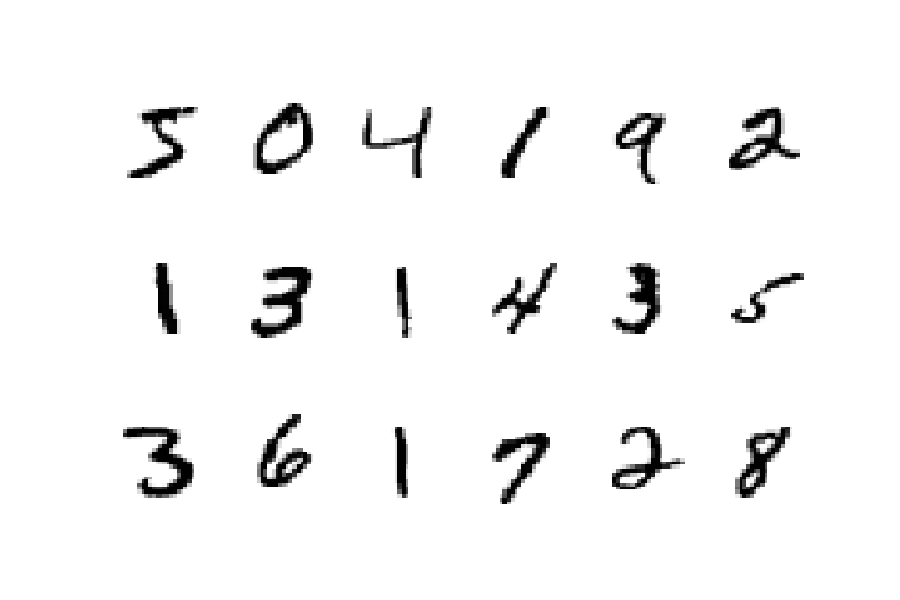
\epsfig{file=Figures/digits.pdf,scale=0.8} 
  \end{center}
  \caption{The first 18 images of the \textsc{Mnist} dataset.}
  \label{fig:mnist_imgs}
\end{figure}

We will use the first $60\,000$ of these images to train a neural network, while the remaining $10\,000$ images
will be used to check the accuracy of the trained network.  As a matter of convenience, the images have been
converted into one large pickled zip files.  You can download this file at the following address:
\\[0.2cm]
\hspace*{1.3cm}
\href{https://github.com/karlstroetmann/Artificial-Intelligence/raw/master/Python/mnist.pkl.gz}{https://github.com/karlstroetmann/Artificial-Intelligence/raw/master/Python/mnist.pkl.gz}
\\[0.2cm]
We will next describe a \textsl{Python} program that loads these images, trains a neural network on it, and
finally evaluates the accuracy of the network.  The program is shown in the Figures
\ref{fig:Digit-Regocnition.ipynb-1}, \ref{fig:Digit-Regocnition.ipynb-2}, \ref{fig:Digit-Regocnition.ipynb-3},
and \ref{fig:Digit-Regocnition.ipynb-4}.


\begin{figure}[!ht]
\centering
\begin{minted}[ frame         = lines, 
                framesep      = 0.3cm, 
                firstnumber   = 1,
                numbers       = left,
                numbersep     = -0.2cm,
                xleftmargin   = 0.8cm,
                xrightmargin  = 0.8cm,
              ]{python3}
    import gzip
    import pickle
    import numpy             as np
    import matplotlib.pyplot as plt
    import random

    def vectorized_result(d):
        e    = np.zeros((10, 1), dtype=np.float32)
        e[d] = 1.0
        return e

    def load_data():
        with gzip.open('mnist.pkl.gz', 'rb') as f:
            train, validate, test = pickle.load(f, encoding="latin1")
        training_inputs   = [np.reshape(x, (784, 1)) for x in train[0]]
        training_results  = [vectorized_result(y) for y in train[1]]
        training_data     = zip(training_inputs, training_results)
        validation_inputs = [np.reshape(x, (784, 1)) for x in validate[0]]
        validation_data   = zip(validation_inputs, validate[1])
        test_inputs       = [np.reshape(x, (784, 1)) for x in test[0]]
        test_data         = zip(test_inputs, test[1])
        training_data     = list(training_data)
        validation_data   = list(validation_data)
        test_data         = list(test_data)
        return (training_data, validation_data, test_data)        

    (training_data, validation_data, test_data) = load_data()
\end{minted}
\vspace*{-0.3cm}
\caption{Code to load the image files.}
\label{fig:Digit-Regocnition.ipynb-1}
\end{figure}
The code on Figure \ref{fig:Digit-Regocnition.ipynb-1} on page \pageref{fig:Digit-Regocnition.ipynb-1} shows the
code to load the image files.  We discuss it line by line.
\begin{enumerate}
\item Since the images are have been compressed as a \texttt{.gz} file, we need the module \texttt{gzip} to
      uncompress the file.
\item The format that has been used to store the images is called
      \href{https://docs.python.org/3.6/library/pickle.html}{pickle}.
      This a binary format that can be used to serialize \textsl{Python} objects into binary strings.  These
      strings can then be stored as files and later be used to restore the corresponding \textsl{Python} objects.  In order
      to read pickled objects, we import the module \texttt{pickle}.
\item The images of the handwritten digits that we are going to import have a size of $28 \times 28$ pixels.
      In this program, we will store the images as \texttt{numpy} arrays of size $28 \cdot 28 = 784$.
\item In order to be able to display these images, we import \texttt{matplotlib}.
\item Every image of a handwritten character is associated with a number $d \in \{0, \cdots, 0\}$.
      We need to transform these numbers into the expected output of our neural network.  This neural network
      will have 10 output nodes corresponding to these digits.  The $k$-th output node will be one
      if the neural network has recognized the digit $k$, while all other output nodes will be $0$.

      The function $\texttt{vectorized\_result}(d)$ takes a digit $d \in \{0,\cdots,9\}$ and returns a
      \texttt{numpy} array \texttt{e} of shape $(10, 1)$ such that $\texttt{e}[d][0]=1$ and $\texttt{e}[j][0]=0$ for
      $j\not=d$.  For example, we have
      \begin{verbatim}
      vectorized_result(2) = array([[0.],
                                    [0.],
                                    [1.],
                                    [0.],
                                    [0.],
                                    [0.],
                                    [0.],
                                    [0.],
                                    [0.],
                                    [0.]], dtype=float32)
      \end{verbatim}
      \vspace*{-0.5cm}
      
      For reasons of efficiency we will only use \blue{single precision floating point numbers}. 
\item The function \texttt{load\_data} reads the file \texttt{mnist.pkl.gz}, uncompresses it,
      and returns three lists:
      \begin{enumerate}
      \item \texttt{training\_data} stores the first $50\,000$ images,
      \item \texttt{validation\_data} holds $10\,000$ images that can be used for the validation of
            hyper-parameters,   
      \item \texttt{test\_data} holds the remaining $10\,000$ images.
      \end{enumerate}
      The images are stored as pairs $(x,y)$: $x$ is a \texttt{numyp} array of shape $(784,1)$ and $y$ is a
      \texttt{numpy} array of shape $(10, 1)$.
\end{enumerate}

\begin{figure}[!ht]
\centering
\begin{minted}[ frame         = lines, 
                framesep      = 0.3cm, 
                firstnumber   = last,
                numbers       = left,
                numbersep     = -0.2cm,
                xleftmargin   = 0.8cm,
                xrightmargin  = 0.8cm,
              ]{python3}
    def rndMatrix(rows, cols):
        return np.random.randn(rows, cols) / np.sqrt(cols)

    def sigmoid(x):
        return 1.0 / (1.0 + np.exp(-x))    
    
    def sigmoid_prime(x):
        s = sigmoid(x)
        return s * (1 - s)
\end{minted}
\vspace*{-0.3cm}
\caption{The constructor of the class $\mathtt{network}$.}
\label{fig:Digit-Regocnition.ipynb-2}
\end{figure}

Figure \ref{fig:Digit-Regocnition.ipynb-2} on page \pageref{fig:Digit-Regocnition.ipynb-2}
shows the implementation of three utility functions.
\begin{enumerate}
\item The function $\mathtt{rndMatrix}(r, c)$ creates a matrix of shape $r, c)$ that is filled with
      random numbers.  These numbers have Gaussian distribution with mean $0$ and variance
      $1/r$.  This function is used to initialize the weight matrices.  It is important that not all weights
      are initialized to the same number, for otherwise they would stay the same and then the different neurons
      would effectively all calculate the same feature instead of different features.  It is also important
      that the weights are not to big for otherwise the associated neurons would \blue{saturate} and their
      learning would be very slow.
\item The function $\texttt{sigmoid}(x)$ computes the sigmoid function.  If $x$ is a number,
      $\texttt{sigmoid}(x)$ computes
      \\[0.2cm]
      \hspace*{1.3cm}
      $\ds S(x) := \frac{1}{1 + \texttt{exp}(-x)}$
      \\[0.2cm]
      If $\mathbf{x}$ is a vector of the form $\mathbf{x} = (x_1,\cdots, x_n)^\top$, we have
      \\[0.2cm]
      \hspace*{1.3cm}
      $S(\mathbf{x}) = \bigl(S(x_1), \cdots, S(x_n)\bigr)^\top$.
\item The function $\texttt{sigmoid\_prime}(x)$ computes the derivative of the sigmoid function.
      The implementation is based on the equation:
      \\[0.2cm]
      \hspace*{1.3cm}
      $S'(x) = S(x) \cdot \bigl(1 - S(x)\bigr)$
      \\[0.2cm]
      $x$ can either be a number or a vector.
\end{enumerate}

\begin{figure}[!ht]
\centering
\begin{minted}[ frame         = lines, 
                framesep      = 0.3cm, 
                firstnumber   = last,
                numbers       = left,
                numbersep     = -0.2cm,
                xleftmargin   = 0.8cm,
                xrightmargin  = 0.8cm,
              ]{python3}
    class Network(object):
        def __init__(self, hiddenSize):
            self.mInputSize  = 28 * 28
            self.mHiddenSize = hiddenSize
            self.mOutputSize = 10
            self.mBiasesH    = np.zeros((self.mHiddenSize, 1))   
            self.mBiasesO    = np.zeros((self.mOutputSize, 1))   
            self.mWeightsH   = rndMatrix(self.mHiddenSize, self.mInputSize)  
            self.mWeightsO   = rndMatrix(self.mOutputSize, self.mHiddenSize) 
    
    def feedforward(self, x):
        AH = sigmoid(self.mWeightsH @ x  + self.mBiasesH) 
        AO = sigmoid(self.mWeightsO @ AH + self.mBiasesO) 
        return AO        
    
    def sgd(self, training_data, epochs, mbs, eta, test_data):
        n_test = len(test_data)
        n      = len(training_data)
        for j in range(epochs):
            random.shuffle(training_data)
            mini_batches = [training_data[k : k+mbs] for k in range(0, n, mbs)]
            for mini_batch in mini_batches:
                self.update_mini_batch(mini_batch, eta)    
            print('Epoch %2d: %d / %d' % (j, self.evaluate(test_data), n_test))
            
    def update_mini_batch(self, mini_batch, eta):
        nabla_BH = np.zeros((self.mHiddenSize, 1))  
        nabla_BO = np.zeros((self.mOutputSize, 1))  
        nabla_WH = np.zeros((self.mHiddenSize, self.mInputSize))
        nabla_WO = np.zeros((self.mOutputSize, self.mHiddenSize))
        for x, y in mini_batch:
            dltNbl_BH, dltNbl_BO, dltNbl_WH, dltNbl_WO = self.backprop(x, y)
            nabla_BH += dltNbl_BH
            nabla_BO += dltNbl_BO
            nabla_WH += dltNbl_WH
            nabla_WO += dltNbl_WO      
        alpha = eta / len(mini_batch)
        self.mBiasesH  -= alpha * nabla_BH
        self.mBiasesO  -= alpha * nabla_BO
        self.mWeightsH -= alpha * nabla_WH
        self.mWeightsO -= alpha * nabla_WO
\end{minted}
\vspace*{-0.3cm}
\caption{The class \texttt{Network}, part \texttt{I}.}
\label{fig:Digit-Regocnition.ipynb-3}
\end{figure}


Figure \ref{fig:Digit-Regocnition.ipynb-3} shows the first part of the class \texttt{Network}.  This class
represents a neural network with one hidden layer. 
\begin{enumerate}
\item The member variable \texttt{mInputSize} specifies the number of input nodes.  The neural network for the
      recognition of handwritten digits has 784 inputs.  These inputs are the grey values of the $28 \times 28$
      pixels that constitute the image of the handwritten digit.
\item The member variable \texttt{mHiddenSize}, specifies the number of neurons in the hidden layer.  We assume that
      there is only one hidden layer.  I have experimented with 30 neurons, 60 neurons and $100$ neurons.
      \begin{enumerate}[(a)]
      \item For 30 neurons, the computation took about 1 minute and 58 seconds and the trained neural network achieved an
            accuracy of $94.8\symbol{37}$.
      \item For 60 neurons, the computation took 2 minutes and 51 seconds the network achieved an accuracy of
            $96.1\symbol{37}$.
      \item If there are 100 neurons in the hidden layer, the computation took 3 minutes and 42 secondsseed and achieved an
            accuracy of $97.8\symbol{37}$.

            For 100 neurons, the number of weights in the hidden layer is $784 \cdot 100 = 78\,400$.
            Therefore, the number of weights is greater than the number of training examples.  Hence,
            we should really use \href{http://neuralnetworksanddeeplearning.com/chap3.html}{regularization} in
            order to prevent over-fitting and increase the accuracy of the network.
      \end{enumerate}
\item The argument \texttt{mOutputSize} specifies the number of output neurons.  For the neural network
      recognizing handwritten digits this number is $10$ since there is an output neuron for every digit.
\item Besides storing the topology of the neural network, the class \texttt{Network} stores the biases and
      weights of all the neurons.  The weights are initialized as random numbers.
      \begin{enumerate}
      \item \texttt{mBiasesH} stores the bias vector of the hidden layer.
      \item \texttt{mBiasesO} stores the bias vector of the output layer.
      \item \texttt{mWeightsH} stores the weight matrix $W^{(2)}$, which specifies the weights connecting the
            input layer with the hidden layer.
      \item \texttt{mWeightsH} stores the weight matrix $W^{(3)}$, which specifies the weights connecting the
            hidden layer with the output layer.
      \end{enumerate}
\item The function \texttt{feedforward} receives an image $\mathbf{x}$ of a digit that is stored as a vector of
      shape $(784,1)$ and computes the output of the
      neural network for this image.  The code is a straightforward implementation of the equations (\ref{eq:FF1}) and (\ref{eq:FF2}).
\item The method \texttt{sgd} implements \blue{stochastic gradient descent}.   It receives 5 arguments.
      \begin{enumerate}
      \item \texttt{training\_data} is a list of pairs of the form $\bigl(\mathbf{x}^{(i)}, \mathbf{y}^{(i)}\bigr)$.
            Here, $\mathbf{x}^{(i)}$ is a vector of dimension $784$.  This vector contains the pixels of an image showing
            one of the handwritten digits from the training set.  $\mathbf{y}^{(i)}$ is the \blue{one-hot encoding} of the digit
            that is shown in the image $\mathbf{x}^{(i)}$.
      \item \texttt{epochs} is the number of iterations of gradient descent.  In order to train the neural network to
            recognize handwritten digits, we will use 30 iterations.
      \item \texttt{mbs} is the size of the mini-batches that are used in stochastic gradient descent.
            I have achieved the fastest learning when I have used a mini-batch size of 10.  Using a mini-batch size
            of 20 was slightly slower, but this parameter seems to be quite uncritical.
      \item \texttt{eta} is the learning rate.
      \item \texttt{test\_data} is the list of test data.  These data are only used to check the accuracy, they are
            not used to determine the weights or biases.
      \end{enumerate}
      The implementation of stochastic gradient descent executes a \texttt{for}-loop that runs \texttt{epoch} number
      of times.  At the beginning of each iteration, the training data are shuffled randomly.  Next, the data is
      chopped up into chunks of size \texttt{mbs}.  These chunks are called \blue{mini-batches}.  The inner
      \texttt{for}-loop iterates over all mini-batches and executes one step of gradient descent that only uses the
      data from the mini-batch.  At the end of each iteration of the outer \texttt{for}-loop, the accuracy of the
      current version of the neural net is printed.
\item The method \texttt{update\_mini\_batch} performs one step of gradient descent for the data from one mini-batch.
      It receives two arguments.
      \begin{enumerate}
      \item \texttt{mini\_batch} is the list of training data that constitute one mini-batch.
      \item \texttt{eta} is the \blue{learning rate}.
      \end{enumerate}
      The implementation of \texttt{update\_mini\_batch} works as follows:
      \begin{enumerate}
      \item First, we initialize the vectors \texttt{nabla\_BH}, \texttt{nabla\_BO} and the matrices
            \texttt{nabla\_WH}, \texttt{nabla\_WO} to contain only zeros.
            \begin{enumerate}[(a)]
            \item \texttt{nabla\_BH} will store the gradient of the bias vector of the hidden layer.
            \item \texttt{nabla\_BO} will store the gradient of the bias vector of the output layer.
            \item \texttt{nabla\_WH} will store the gradient of the weight matrix of the hidden layer.
            \item \texttt{nabla\_WO} will store the gradient of the weight matrix of the output layer.
            \end{enumerate}
      \item Next, we iterate of all training examples in the mini-batch and for every training example
            \texttt{[x,y]} we compute the contribution of this training example to the gradients of the
            cost function $C$, i.e.~we compute
            \\[0.2cm]
            \hspace*{1.3cm}
            $\nabla_{\mathbf{b}^{(l)}} C_{\mathbf{x}, \mathbf{y}}$ \quad and \quad  $\nabla_{W^{(l)}} C_{\mathbf{x},
              \mathbf{y}}$ 
            \\[0.2cm]
            for the hidden layer and the output layer.  These gradients are computed by the function
            \texttt{backprop}.
      \item Finally, the bias vectors and the weight matrices are updated according to the learning rate and the
            computed gradients.
      \end{enumerate}
\end{enumerate}

\begin{figure}[!ht]
\centering
\begin{minted}[ frame         = lines, 
                framesep      = 0.3cm, 
                firstnumber   = last,
                numbers       = left,
                numbersep     = -0.2cm,
                xleftmargin   = 0.5cm,
                xrightmargin  = 0.5cm,
              ]{python3}
        def backprop(self, x, y):
            # feedforward pass
            ZH = self.mWeightsH @ x  + self.mBiasesH
            AH = sigmoid(ZH)
            ZO = self.mWeightsO @ AH + self.mBiasesO
            AO = sigmoid(ZO)
            # backwards pass, output layer
            epsilonO = (AO - y) # * sigmoid_prime(ZO)
            nabla_BO = epsilonO
            nabla_WO = epsilonO @ AH.transpose()
            # backwards pass, hidden layer
            epsilonH = (self.mWeightsO.transpose() @ epsilonO) * sigmoid_prime(ZH)
            nabla_BH = epsilonH
            nabla_WH = epsilonH @ x.transpose()
            return (nabla_BH, nabla_BO, nabla_WH, nabla_WO)
        
        def evaluate(self, test_data):
            test_results = [(np.argmax(self.feedforward(x)), y) for (x, y) in test_data]
            return sum(int(y1 == y2) for (y1, y2) in test_results)
        # end of class Network
            
    net = Network(60)
    net.sgd(training_data, 30, 20, 0.3, test_data)   
\end{minted}
\vspace*{-0.3cm}
\caption{The class \texttt{Network}, part \texttt{II}.}
\label{fig:Digit-Regocnition.ipynb-4}
\end{figure}


The method \texttt{backprop} that is shown in Figure \ref{fig:Digit-Regocnition.ipynb-4} computes the gradients
of the bias vectors and the weight matrices with respect to 
a single training example $\langle \texttt{x}, \texttt{y} \rangle$.  The implementation of \texttt{backprop}
proceeds as follows:
\begin{enumerate}
\item First, the vector \texttt{ZH} is computed according to the formula
      \\[0.2cm]
      \hspace*{1.3cm}
      $\mathbf{z}^{(2)} = W^{(2)} \cdot \mathbf{x} + \mathbf{b}^{(2)}$.
      \\[0.2cm]
      Here, $W^{(2)}$ is the weight matrix of the hidden layer that is stored in \texttt{mWeightsH}, while
      $\mathbf{b}^{(2)}$ is the bias vector of the hidden layer.  This vector is stored in \texttt{mBiasesH}.
\item The activation of the neurons in the hidden layer \texttt{AH} is computed by applying the sigmoid
      function to the vector $\mathbf{z}^{(2)}$.
\item Next, the vector \texttt{ZH} is computed according to the formula
      \\[0.2cm]
      \hspace*{1.3cm}
      $\mathbf{z}^{(3)} = W^{(3)} \cdot \mathbf{x} + \mathbf{b}^{(3)}$.
      \\[0.2cm]
      Here, $W^{(3)}$ is the weight matrix of the output layer that is stored in \texttt{mWeightsO}, while
      $\mathbf{b}^{(3)}$ is the bias vector of the output layer.  This vector is stored in \texttt{mBiasesO}.
\item The activation of the neurons in the output layer \texttt{AO} is computed by applying the sigmoid
      function to the vector $\mathbf{z}^{(3)}$.

      These four step constitute the forward pass of backpropagation.
\item Next, the error in the output layer \texttt{epsilonO} is computed using the backpropagation equation
      (BP1v)
      \\[0.2cm]
      \hspace*{1.3cm}
      $\ds \boldsymbol{\varepsilon}^{(3)} = (\mathbf{a}^{(3)} - \mathbf{y}) \odot S'\bigl(\mathbf{z}^{(3)}\bigr)$.
\item According to  equation (BP3v), the gradient of the cost function with respect to the bias vector of the
      output layer is given as
      \\[0.2cm]
      \hspace*{1.3cm}
      $\ds \nabla_{\mathbf{b}^{(3)}} C_{\mathbf{x}, \mathbf{y}} = \boldsymbol{\varepsilon}^{(3)}$.
      \\[0.2cm]
      This gradient is stored in the variable \texttt{nabla\_BO}.
\item According to equation (BP4v), the gradient  of the cost function with respect to the weight matrix of the
      output layer is given as
      \\[0.2cm]
      \hspace*{1.3cm}
      $\ds \nabla_{W^{(3)}} C_{\mathbf{x}, \mathbf{y}} = \boldsymbol{\varepsilon}^{(3)} \cdot \bigl(\mathbf{a}^{(2)}\bigr)^\top$.
      \\[0.2cm]
      This gradient is stored in the variable \texttt{nabla\_WO}.
\item Next, the error in the hidden layer \texttt{epsilonH} is computed using the backpropagation equation
      (BP2v)
      \\[0.2cm]
      \hspace*{1.3cm}
      $\ds \boldsymbol{\varepsilon}^{(2)} = \Bigl(\bigl(W^{(3)}\bigr)^\top \cdot \boldsymbol{\varepsilon}^{(3)}\Bigr) \odot
           S'\bigl(\mathbf{z}^{(2)}\bigr)
      $.
\item Finally, the gradients of the cost function with respect to the bias
      vector and the weight matrix of the hidden layer are computed.  This is completely to the computation of
      the corresponding gradients of the output layer.
\item The method \texttt{evaluate} is used to evaluate the accuracy of the neural network on the test data.
\item Finally, we see how the computation can be started by creating an object of class \texttt{Network} and
      then calling the method \texttt{sgd}.
\end{enumerate}
The program discussed in this section is available as a jupyter notebook at the following address:
\\[0.2cm]
\hspace*{0.3cm}
\href{https://github.com/karlstroetmann/Artificial-Intelligence/blob/master/Python/Digit-Recognition.ipynb}{https://github.com/karlstroetmann/Artificial-Intelligence/blob/master/Python/Digit-Recognition.ipynb}.





%%% Local Variables:
%%% mode: latex
%%% TeX-master: "artificial-intelligence"
%%% End:
